% Soubory musí být v kódování, které je nastaveno v příkazu \usepackage[...]{inputenc}

\documentclass[%        Základní nastavení
  %draft,    				  % Testovací překlad
  12pt,       				% Velikost základního písma je 12 bodů
	t,                  % obsah slajdů bude vždy začínat od shora (nebude vertikálně centrovaný)
	aspectratio=1610,   % poměr stran bude 16:10 (všechny projektory v učebnách na Technické 12 Brno),
	                    % další volby jsou 43, 149, 169, 54, 32.
	unicode,						% Záložky a informace budou v kódování unicode
]{beamer}				    	% Dokument třídy 'zpráva', vhodná pro sazbu závěrečných prací s kapitolami
%\usepackage{etex}

\usepackage{graphicx} % Balíček 'graphicx' pro vkládání obrázků
											% Nutné pro vložení logotypů školy a fakulty

\usepackage[          % Balíček 'acronym' pro sazby zkratek a symbolů
	nohyperlinks				% Nebudou tvořeny hypertextové odkazy do seznamu zkratek
]{acronym}						
											% Nutné pro použití prostředí 'acronym' balíčku 'thesis'

%% Balíček hyperref je volán třídou beamer automaticky, proto není třeba následujícího kódu:
%\usepackage[
%	breaklinks=true,		% Hypertextové odkazy mohou obsahovat zalomení řádku
%	hypertexnames=false % Názvy hypertextových odkazů budou tvořeny
%											% nezávisle na názvech TeXu
%]{hyperref}						% Balíček 'hyperref' pro sazbu hypertextových odkazů
%											% Nutné pro použití příkazu 'nastavenipdf' balíčku 'thesis'

\usepackage{cmap} 		% Balíček cmap zajišťuje, že PDF vytvořené `pdflatexem' je
											% plně "prohledávatelné" a "kopírovatelné"

%\usepackage{upgreek}	% Balíček pro sazbu stojatých řeckých písmem
											%% např. stojaté pí: \uppi
											%% např. stojaté mí: \upmu (použitelné třeba v mikrometrech)
											%% pozor, grafická nekompatibilita s fonty typu Computer Modern!

%\usepackage{amsmath} %balíček pro sabu náročnější matematiky

\usepackage{booktabs} % Balíček, který umožňuje v tabulce používat
                      % příkazy \toprule, \midrule, \bottomrule


%%%%%%%%%%%%%%%%%%%%%%%%%%%%%%%%%%%%%%%%%%%%%%%%%%%%%%%%%%%%%%%%%
%%%%%%      Definice informací o dokumentu             %%%%%%%%%%
%%%%%%%%%%%%%%%%%%%%%%%%%%%%%%%%%%%%%%%%%%%%%%%%%%%%%%%%%%%%%%%%%

% V tomto souboru se nastavují téměř veškeré informace, proměnné mezi studenty:
% jméno, název práce, pohlaví atd.
% Tento soubor je SDÍLENÝ mezi textem práce a prezentací k obhajobě -- netřeba něco nastavovat na dvou místech.

\usepackage[
%%% Z následujících voleb jazyka lze použít pouze jednu
  czech-english,		% originální jazyk je čeština, překlad je anglicky (výchozí)
  %english-czech,	% originální jazyk je angličtina, překlad je česky
  %slovak-english,	% originální jazyk je slovenština, překlad je anglicky
  %english-slovak,	% originální jazyk je angličtina, překlad je slovensky
%
%%% Z následujících voleb typu práce lze použít pouze jednu
  semestral,		  % semestrální práce (nesází se abstrakty, prohlášení, poděkování) (výchozí)
  %bachelor,			%	bakalářská práce
  %master,			  % diplomová práce
  %treatise,			% pojednání o disertační práci
  %doctoral,			% disertační práce
%
%%% Z následujících voleb zarovnání objektů lze použít pouze jednu
%  left,				  % rovnice a popisky plovoucích objektů budou zarovnány vlevo
	center,			    % rovnice a popisky plovoucích objektů budou zarovnány na střed (vychozi)
%
]{thesis}   % Balíček pro sazbu studentských prací


%%% Jméno a příjmení autora ve tvaru
%  [tituly před jménem]{Křestní}{Příjmení}[tituly za jménem]
% Pokud osoba nemá titul před/za jménem, smažte celý řetězec '[...]'
\author[Bc.]{Viktor}{Slezák}

%%% Identifikační číslo autora (VUT ID)
\butid{203745}

%%% Pohlaví autora/autorky
% (nepoužije se ve variantě english-czech ani english-slovak)
% Číselná hodnota: 1...žena, 0...muž
\gender{0}

%%% Jméno a příjmení vedoucího/školitele včetně titulů
%  [tituly před jménem]{Křestní}{Příjmení}[tituly za jménem]
% Pokud osoba nemá titul před/za jménem, smažte celý řetězec '[...]'
\advisor[Ing.]{Matěj}{Ištvánek}

%%% Jméno a příjmení oponenta včetně titulů
%  [tituly před jménem]{Křestní}{Příjmení}[tituly za jménem]
% Pokud osoba nemá titul před/za jménem, smažte celý řetězec '[...]'
% Nastavení oponenta se uplatní pouze v prezentaci k obhajobě;
% v případě, že nechcete, aby se na titulním snímku prezentace zobrazoval oponent, pouze příkaz zakomentujte;
% u obhajoby semestrální práce se oponent nezobrazuje (jelikož neexistuje)
% U dizertační práce jsou typicky dva až tři oponenti. Pokud je chcete mít na titulním slajdu, prosím ručně odkomentujte a upravte jejich jména v definici "VUT title page" v souboru thesis.sty.
\opponent[doc.\ Mgr.]{Křestní}{Příjmení}[Ph.D.]

%%% Název práce
%  Parametr ve složených závorkách {} je název v originálním jazyce,
%  parametr v hranatých závorkách [] je překlad (podle toho jaký je originální jazyk).
%  V případě, že název Vaší práce je dlouhý a nevleze se celý do zápatí prezentace, použijte příkaz
%  \def\insertshorttitle{Zkác.\ náz.\ práce}
%  kde jako parametr vyplníte zkrácený název. Pokud nechcete zkracovat název, budete muset předefinovat,
%  jak se vytváří patička slidu. Viz odkaz: https://bit.ly/3EJTp5A
\title[Light animations for the Spectoda system based on the analysis of parameters from music recordings]{Světelné animace pro systém Spectoda na základě analýzy parametrů z hudebních nahrávek}

%%% Označení oboru studia
%  Parametr ve složených závorkách {} je název oboru v originálním jazyce,
%  parametr v hranatých závorkách [] je překlad
\specialization[Audio engineering]{Audio inženýrství}

%%% Označení ústavu
%  Parametr ve složených závorkách {} je název ústavu v originálním jazyce,
%  parametr v hranatých závorkách [] je překlad
%\department[Department of Control and Instrumentation]{Ústav automatizace a měřicí techniky}
%\department[Department of Biomedical Engineering]{Ústav biomedicínského inženýrství}
%\department[Department of Electrical Power Engineering]{Ústav elektroenergetiky}
%\department[Department of Electrical and Electronic Technology]{Ústav elektrotechnologie}
%\department[Department of Physics]{Ústav fyziky}
%\department[Department of Foreign Languages]{Ústav jazyků}
%\department[Department of Mathematics]{Ústav matematiky}
%\department[Department of Microelectronics]{Ústav mikroelektroniky}
%\department[Department of Radio Electronics]{Ústav radioelektroniky}
%\department[Department of Theoretical and Experimental Electrical Engineering]{Ústav teoretické a experimentální elektrotechniky}
\department[Department of Telecommunications]{Ústav telekomunikací}
%\department[Department of Power Electrical and Electronic Engineering]{Ústav výkonové elektrotechniky a elektroniky}

%%% Označení fakulty
%  Parametr ve složených závorkách {} je název fakulty v originálním jazyce,
%  parametr v hranatých závorkách [] je překlad
%\faculty[Faculty of Architecture]{Fakulta architektury}
\faculty[Faculty of Electrical Engineering and~Communication]{Fakulta elektrotechniky a~komunikačních technologií}
%\faculty[Faculty of Chemistry]{Fakulta chemická}
%\faculty[Faculty of Information Technology]{Fakulta informačních technologií}
%\faculty[Faculty of Business and Management]{Fakulta podnikatelská}
%\faculty[Faculty of Civil Engineering]{Fakulta stavební}
%\faculty[Faculty of Mechanical Engineering]{Fakulta strojního inženýrství}
%\faculty[Faculty of Fine Arts]{Fakulta výtvarných umění}
%
%Nastavení logotypu (v hranatych zavorkach zkracene logo, ve slozenych plne):
\facultylogo[logo/FEKT_zkratka_barevne_PANTONE_CZ]{logo/UTKO_color_PANTONE_CZ}

%%% Rok odevzdání práce
\graduateyear{2023}
%%% Akademický rok odevzdání práce
\academicyear{2023/24}

%%% Datum obhajoby (uplatní se pouze v prezentaci k obhajobě)
\date{11.\,11.\,1980} 

%%% Místo obhajoby
% Na titulních stránkách bude automaticky vysázeno VELKÝMI písmeny (pokud tyto stránky sází šablona)
\city{Brno}

%%% Abstrakt
\abstract[%
In this paper, is explored the field of Music Information Retrieval. Based on the knowledge acquired, a system structure for generating animations from parameters of a music recording is proposed. Furthermore, the possibilities for extracting these parameters are described and compared.
]{%
V práci je prozkoumána problematika oboru Music information retrieval. Na základě získaných znalostí je navržena struktura systému pro generování animací z parametrů hudební nahrávky. Dále jsou popsány a porovnány možnosti jak tyto parametry extrahovat.
}

%%% Klíčová slova
\keywrds[%
MIR, feature extraction, audio analysis, animation generator
]{%
MIR, extrakce parametrů, audio analýza, generátor animací
}

%%% Poděkování
\acknowledgement{%
Rád bych poděkoval vedoucímu diplomové práce
panu Ing. Matěj Ištvánek\ za odborné vedení,
konzultace, trpělivost a~podnětné návrhy k~práci.
}%      % v tomto souboru doplňte údaje o sobě, o názvu práce...
                       % (tento soubor je sdílený s textem práce)
	\usepackage[utf8]		  %	Kódování zdrojových souborů je UTF-8
	{inputenc}					% Balíček pro nastavení kódování zdrojových souborů
\usepackage{fontspec}

%%%%%%%%%%%%%%%%%%%%%%%%%%%%%%%%%%%%%%%%%%%%%%%%%%%%%%%%%%%%%%%%%%%%%%%%

%%%%%%%%%%%%%%%%%%%%%%%%%%%%%%%%%%%%%%%%%%%%%%%%%%%%%%%%%%%%%%%%%%%%%%%%
%%%%%%     Nastavení polí ve Vlastnostech dokumentu PDF      %%%%%%%%%%%
%%%%%%%%%%%%%%%%%%%%%%%%%%%%%%%%%%%%%%%%%%%%%%%%%%%%%%%%%%%%%%%%%%%%%%%%
%% Při vloženém balíčku 'hyperref' lze použít příkaz '\pdfsettings'
\pdfsettings
%  Nastavení polí je možné provést také ručně příkazem:
%\hypersetup{
%  pdftitle={Název studentské práce},    	% Pole 'Document Title'
%  pdfauthor={Autor studenstké práce},   	% Pole 'Author'
%  pdfsubject={Typ práce}, 						  	% Pole 'Subject'
%  pdfkeywords={Klíčová slova}           	% Pole 'Keywords'
%}
\hypersetup{pdfpagemode=FullScreen}       % otevření rovnou v režimu celé obrazovky
%%%%%%%%%%%%%%%%%%%%%%%%%%%%%%%%%%%%%%%%%%%%%%%%%%%%%%%%%%%%%%%%%%%%%%%

\usetheme{VUT} 				% barvy a rozložení prezentace odpovídající VUT FEKT
% alternativně lze použít jiná berevná témata, ale bez záruky. Například: 
%\usetheme{Darmstadt} \usecolortheme{default2}
\logoheader					% vytvoření zkráceného loga VUT FEKT v hlavičce slajdu, nechte odkomentované



\begin{document}

% v případě zakomentování následujícího se zobrazí v pravém dolním rohu slajdů klikatelné navigační symboly 
\disablenavigationsymbols

% titulní snímek, vysazen bez horních, dolních a postranních lišt (volba plain),
% není tak vysazen ani nadpis snímku
\maketitle

%%%%%%%%%%%%%%%%%%%%%%%%%%%%%%%%%%%%%%%%%%%%%%%%%%%%%%%%%%%%%%%%%%%%%%%
% 1. snímek s cíli (zadaním) práce
\begin{frame} 
	% nadpis snímku

% 1. Teoretický průzkum
% 2. Návrh struktruy výsledného systému
% 3. Výběr vhodných metod pro získání parametrů jejich realizace a porovnání

	\frametitle{Cíle práce}
	\begin{block}{Návrh struktruy algoritmu pro generování světelných animací}
		\begin{itemize}
			\item Teoretický průzkum	
			\begin{itemize}
				\item Výzkumů v oblasti Music information retrieval
				\item Možností analýzy parametrů hudební nahrávky
				\item Dostupná řešení extrakce parametrů z hudební nahrávky
			\end{itemize}
			\item Výběr vhodných parametrů
			\item Návrh postupu generování animací na zákaldě vybraných parametrů
		\end{itemize}
	\end{block}
	\begin{block}{Realizace}
		\begin{itemize}
			\item Extrakce parametrů pomocí dostupných metod
			\item Porovnání získaných parametrů a zhodnocení metod
		\end{itemize}
	\end{block}
\end{frame}

%%%%%%%%%%%%%
\begin{frame} 
	\frametitle{Úvod do problematiky}
	\begin{itemize}
		\item Automatické generování animací s dostatečným množstvím času.
	\end{itemize}

	% \begin{block}{Generování světelných animací}
	% 	\begin{itemize}
	% 		\item Z pohledu času
	% 		\begin{itemize}
	% 			\item V minulosti
	% 			\item V reálném čase
	% 		\end{itemize}
	% 		\item Z pohledu způsobu
	% 		\begin{itemize}
	% 			\item navržené člověkem
	% 			\item navržené strojem
	% 		\end{itemize}
	% 	\end{itemize}
	% \end{block}

	\begin{block}{Parametry}
		\begin{itemize}
			\item Jaké parametry využít?
			\item Co tyto parametry ovlivňůjí? 
			\item Jakým způsobem jsou paramety získány?
		\end{itemize}
	\end{block}
\end{frame} 

\begin{frame}
	\frametitle{Výběr}
	Vybrané parametry hudební nahrávky pro generování světelných animací.
	\begin{columns}[T]
		\begin{column}{0.3\textwidth}		% první sloupec
			\begin{itemize}
				\item Detekce dob
				\item Chroma vektory
				\item Tempo
				\item Efektivní hodnota 
				\item Segmenty
				\item Žánr
				\item Nálada
			\end{itemize}
		\end{column}
		\begin{column}{0.7\textwidth}		
			% 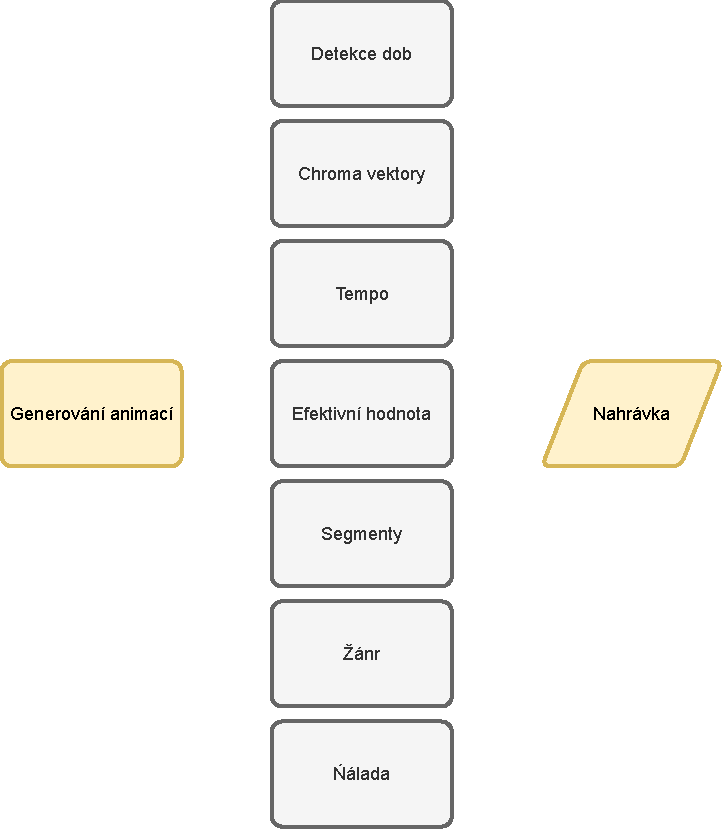
\includegraphics[width = 0.6\columnwidth]{obrazky/Prez_parametry.pdf}
		\end{column}
		
	\end{columns}
\end{frame}

\begin{frame}
	\frametitle{Využití}
	\begin{block}{Výběr datasetu}
	\end{block}
	\vspace{1cm}

	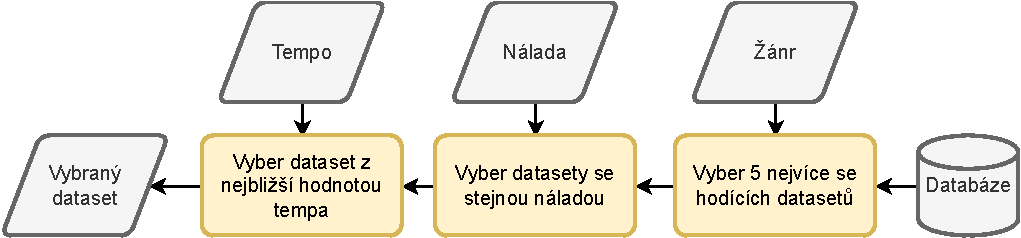
\includegraphics[width = 1\columnwidth]{obrazky/Dataset_selection_diagram.pdf}

\end{frame}

\begin{frame}
	\frametitle{Využití}
	\begin{block}{Umístění bloků animací v čase}
		\begin{itemize}
			\item Začátek dle dob
			\item Délka dle tempa a efektivní hodnoty
			\item Konec dle délky animace zaorkouhlené na nejbližší dobu
		\end{itemize}
	\end{block}
	\begin{block}{Výběr bloku animace}
		\begin{itemize}
			\item Výběr na základě efektivní hodnoty v čase bloku animace
		\end{itemize}
	\end{block}

	\begin{block}{Barevná paleta}
		\begin{itemize}
			\item Vytvoření palety barev z analýzy chromavektorů nahrávky
			\item Určení znějících tónů v čase bloku animace z chromavektorů
			\item Přiřazení bloku animace barvy dle tónů a palety barev
		\end{itemize}
	\end{block}
\end{frame}

% \begin{frame}
% 	\frametitle{}
% 	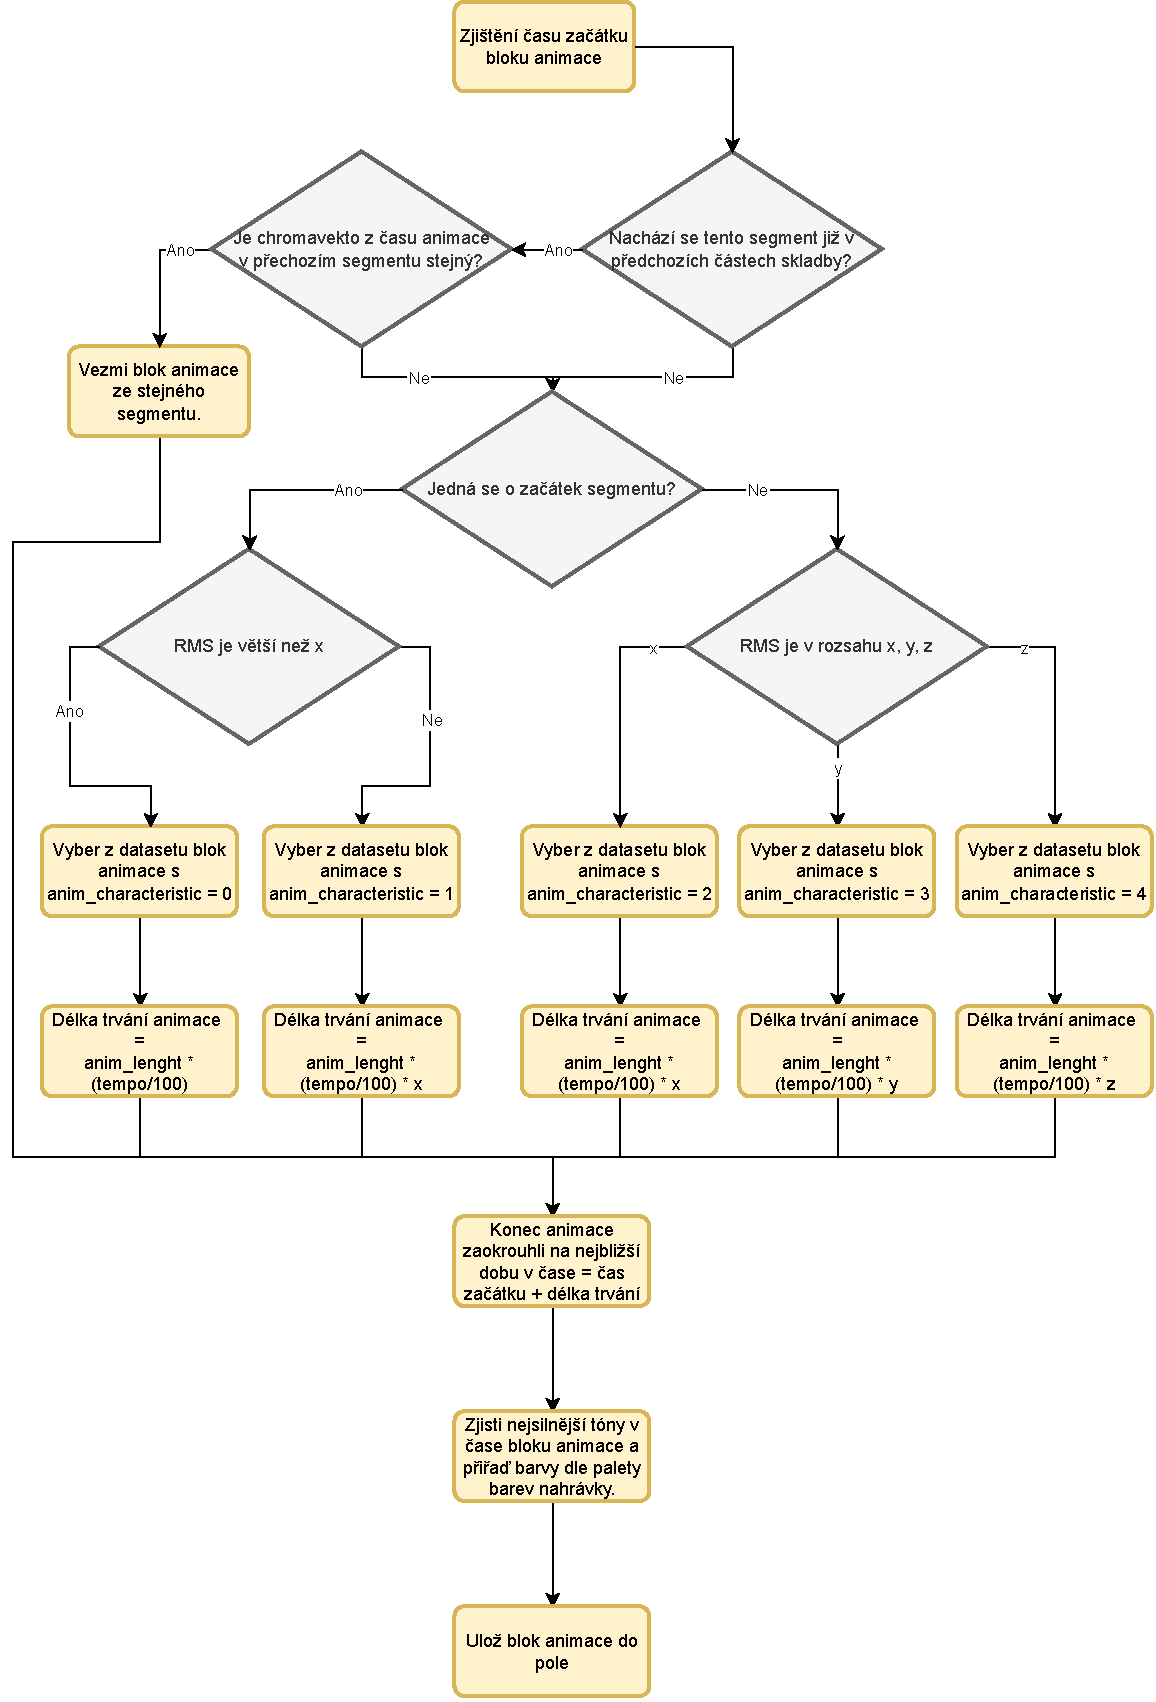
\includegraphics[width = 0.4\columnwidth]{obrazky/Logical_structure_diagram.pdf}
% \end{frame}

\begin{frame}
	\frametitle{Extrakce}
	\begin{block}{Využité knihovny}
		\begin{itemize}
			\item Librosa
				\begin{itemize}
					\item Detekce dob a tempa
					\item Analýza chromavektorů
					\item Výpočet efektivní hodnoty
				\end{itemize}
			\item Madmom
				\begin{itemize}
					\item Detekce dob a tempa
					\item Analýza chromavektorů
				\end{itemize}
			\item Aubio
				\begin{itemize}
					\item Detekce dob a tempa
				\end{itemize}
			\item Mir\_eval
				\begin{itemize}
					\item Výpočet Cemgil skóré pro porovnání detekce dob
				\end{itemize}
		\end{itemize}
	\end{block}
	% Použité knihovny metody 
	% Hodnocení metod a posání výsledků
\end{frame}

\begin{frame}
	\frametitle{}
	\centering
	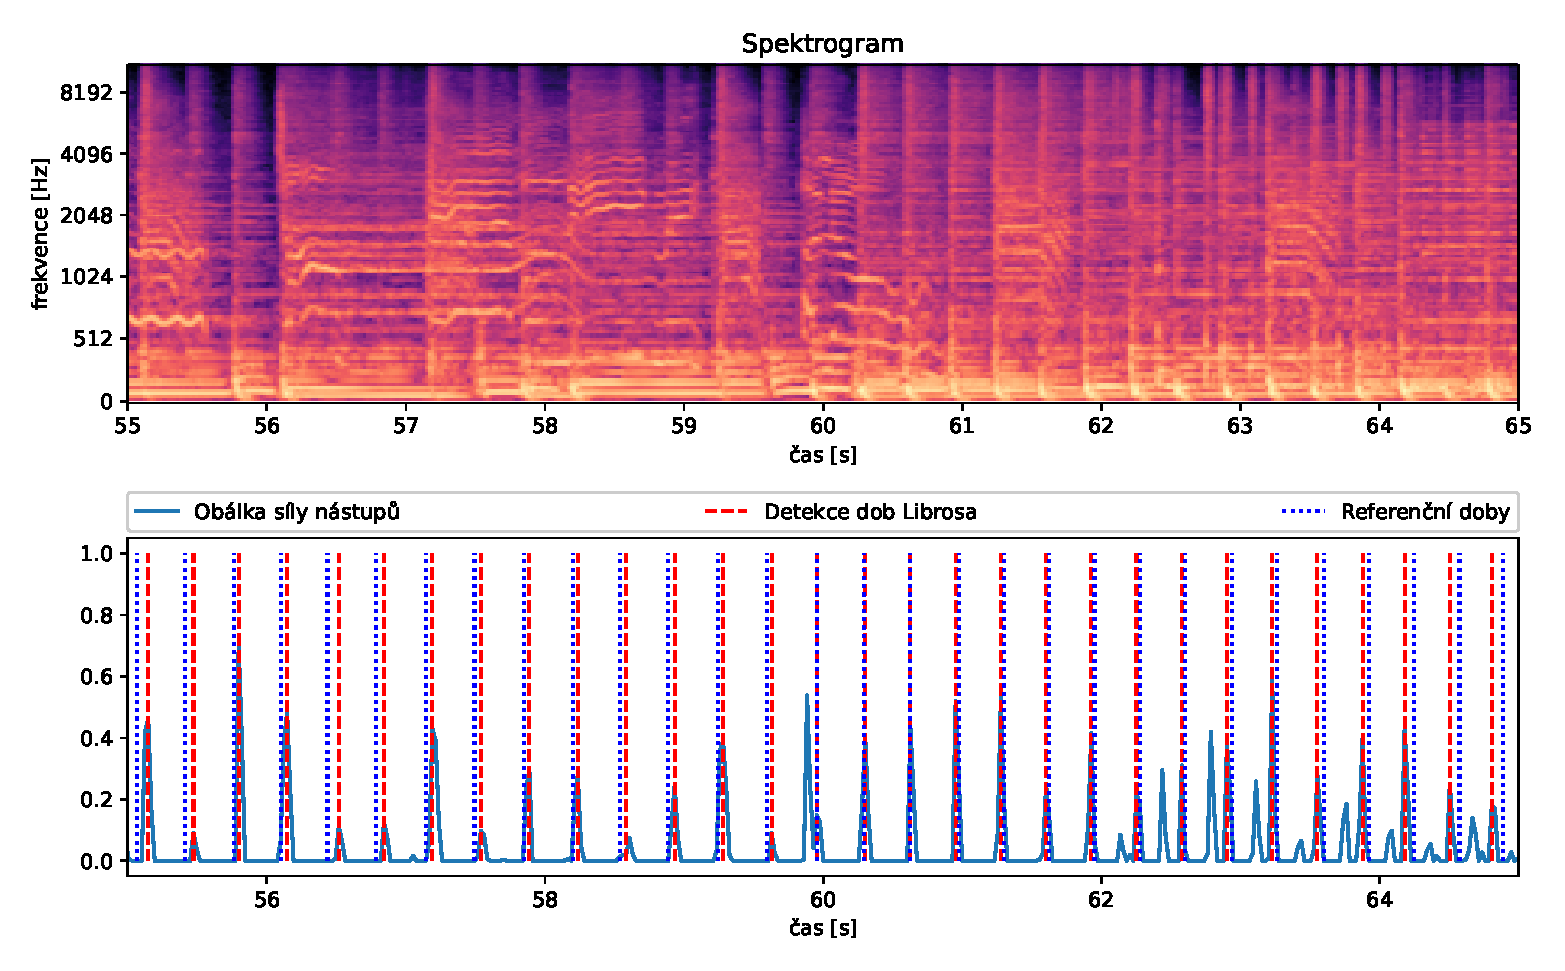
\includegraphics[width = 1\columnwidth]{obrazky/Beat_track_presentation.eps}
\end{frame}

\begin{frame}
	\frametitle{}
	\centering
	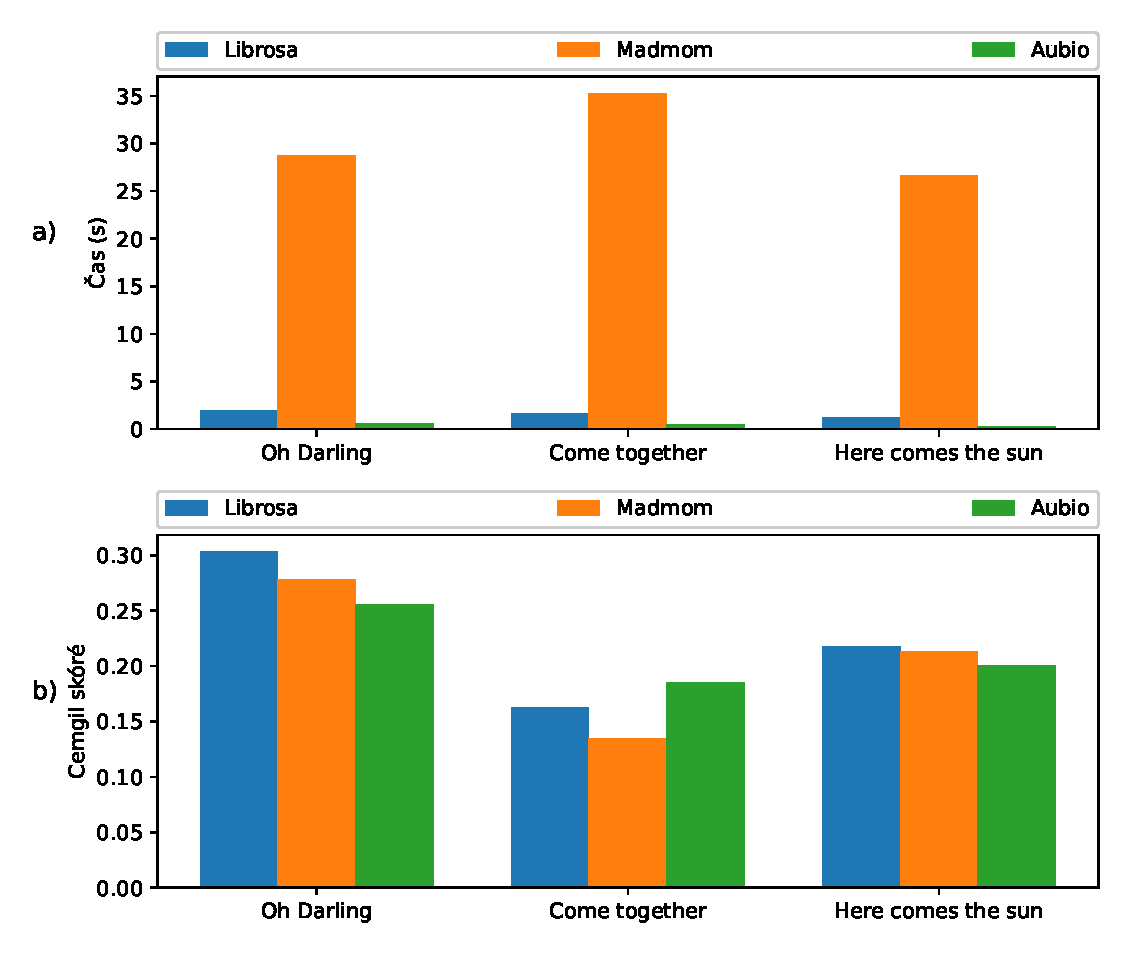
\includegraphics[width = 0.75\columnwidth]{obrazky/Beat_tracking_time_and_cemgil_graphs.eps}
\end{frame}

\begin{frame}
	\frametitle{}
	\centering
	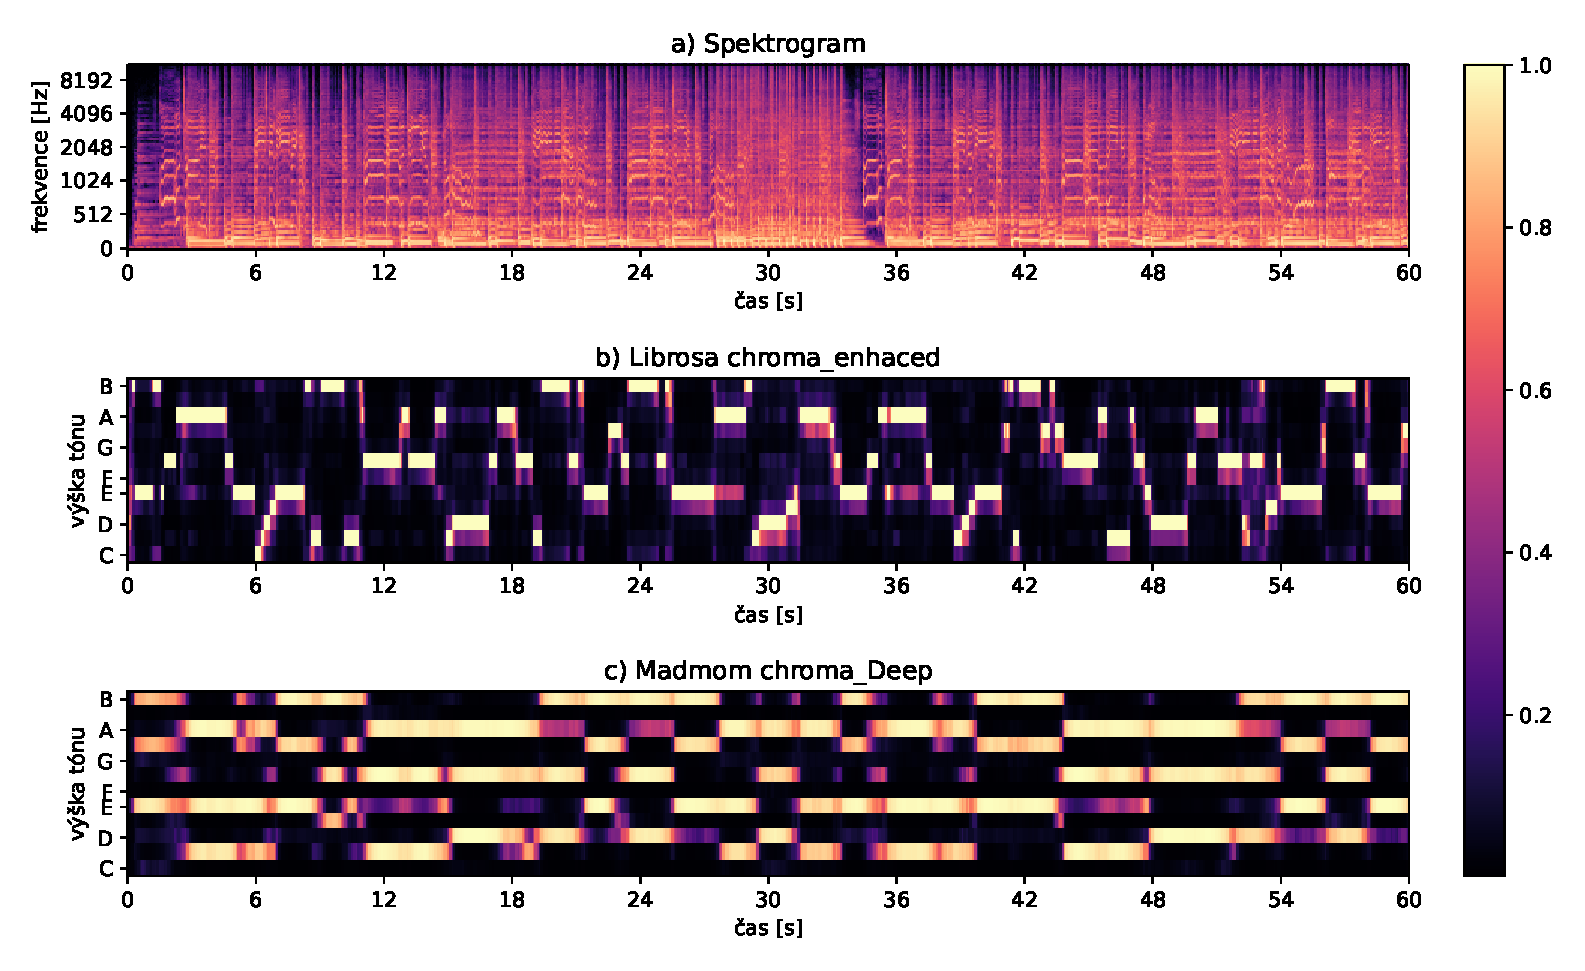
\includegraphics[width = 1\columnwidth]{obrazky/Chromavector_presentation.eps}
\end{frame}

\begin{frame}
	\frametitle{}
	\centering
	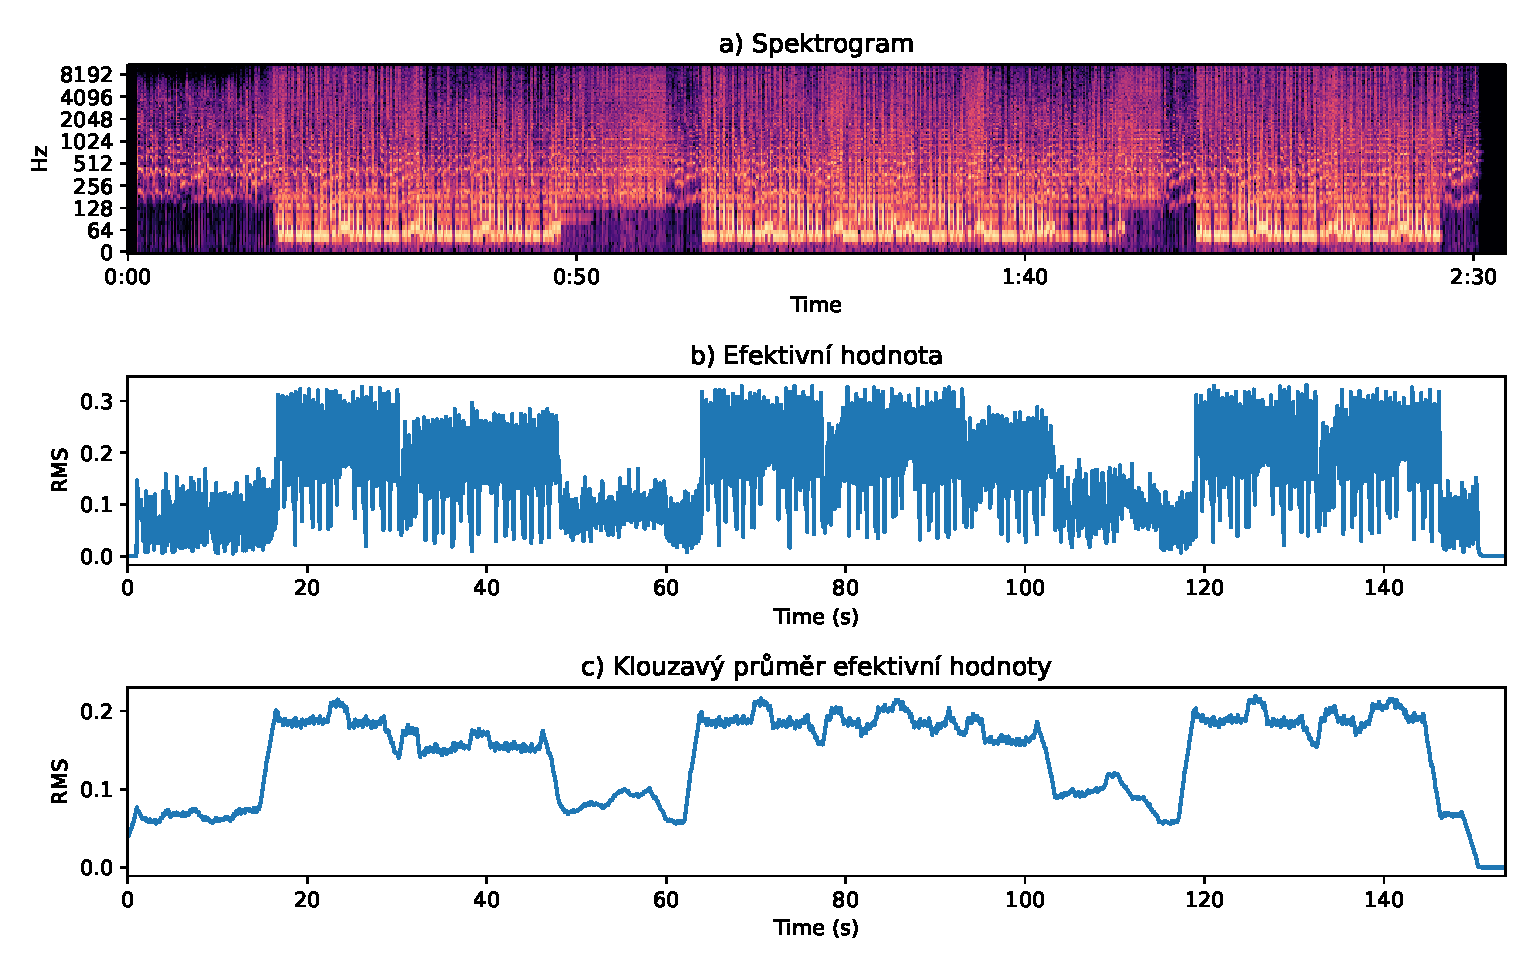
\includegraphics[width = 1\columnwidth]{obrazky/Belly_dancer_RMS.eps}
\end{frame}


% Shrnutí (přídána obálka síly nástupu)

\begin{frame} 
	\frametitle{Závěr}
	\begin{block}{Splnění cílů}
		\begin{itemize}
			\item Teoretický průzkum
			\item Návrh struktury výsledného algoritmu
			\item Extrakce a porovnání parametrů
		\end{itemize}
	\end{block}
	\begin{block}{Diplomová práce a návrhy na zlepšení}
		\begin{itemize}
			\item Segmentace nahrávky
			\item Rozpoznávání žánrů
			\item Využití obálky síly nástupů
			\item Realizace a optimalizace funkčního systému pro generování animací
		\end{itemize}
	\end{block}
\end{frame}

% podekovani
\begin{frame}[c] 
% bez nadpisu snímku
	\frametitle{\mbox{ }}
	\begin{center}
		{\Huge Děkuji za pozornost!}
	\end{center}
\end{frame}

\end{document}
